\documentclass[11pt]{article}
\usepackage[margin=1.4cm]{geometry}
\usepackage{amsmath}
\usepackage{amssymb}
\usepackage{enumitem}
\usepackage{titlesec}
\usepackage{xcolor}
\usepackage{fancyhdr}
\usepackage{tikz}
\usepackage{multicol}
\usetikzlibrary{arrows.meta,positioning}
\usepackage{array}

\setlength{\columnsep}{0.8cm}
\setlength{\columnseprule}{0.4pt}
\renewcommand{\arraystretch}{1.3}
\raggedcolumns

\pagestyle{fancy}
\setlength{\headheight}{14pt}
\fancyhf{}
\fancyhead[L]{Year 9 Mathematics}
\fancyhead[R]{Linear Number Patterns -- Extra Practice}
\fancyfoot[C]{\thepage}
\renewcommand{\headrulewidth}{0.4pt}

\titleformat{\section}{\normalsize\bfseries\color{blue!50!black}}{\thesection}{0.5em}{}

\newcommand{\ans}{\hrulefill}
\newcommand{\anshere}{\par\vspace{0.2em}\noindent\ans\par\vspace{0.2em}}
\newcommand{\ansprose}{\par\vspace{0.2em}\noindent\ans\par\vspace{0.4em}\noindent\ans\par\vspace{0.2em}}
% #1 = top-left row label, #2 = bottom-left row label, #3 = number of data
% columns, #4 = comma list of #3 header values (use {} for a blank header).
% Draws the value table, then a row of boxes offset by half a column and
% tied to the table above by tick marks at each internal column boundary.
\newcommand{\patterntable}[4]{%
  \par\noindent\begin{tikzpicture}[line width=0.8pt, baseline=0pt]
    \def\cw{0.85}\def\lw{0.85}\def\rh{0.72}\def\gap{0.32}
    \pgfmathtruncatemacro{\Nn}{#3}
    \pgfmathtruncatemacro{\Nmo}{\Nn-1}
    \pgfmathtruncatemacro{\Nmt}{\Nn-2}
    \draw (0,0) rectangle ({\lw+\Nn*\cw},{2*\rh});
    \draw (0,\rh) -- ({\lw+\Nn*\cw},\rh);
    \draw (\lw,0) -- (\lw,{2*\rh});
    \foreach \i in {1,...,\Nn} { \draw ({\lw+\i*\cw},0) -- ({\lw+\i*\cw},{2*\rh}); }
    \node at ({\lw/2},{1.5*\rh}) {#1};
    \node at ({\lw/2},{0.5*\rh}) {#2};
    \foreach \val [count=\i] in {#4} { \node at ({\lw+(\i-0.5)*\cw},{1.5*\rh}) {\val}; }
    \draw ({\lw+0.5*\cw},{-\gap-\rh}) rectangle ({\lw+(\Nn-0.5)*\cw},{-\gap});
    \foreach \j in {1,...,\Nmt} { \draw ({\lw+(0.5+\j)*\cw},{-\gap-\rh}) -- ({\lw+(0.5+\j)*\cw},{-\gap}); }
    \foreach \k in {1,...,\Nmo} { \draw ({\lw+\k*\cw},0) -- ({\lw+\k*\cw},{-\gap}); }
  \end{tikzpicture}\par\vspace{0.3em}%
}
\newcommand{\drawbox}[1]{%
  \par\noindent\fbox{%
    \begin{minipage}[t][#1][t]{\dimexpr\linewidth-2\fboxsep-2\fboxrule}
      \vspace{0.15em}\hspace{0.15em}\textit{\scriptsize Draw your pattern here.}
    \end{minipage}%
  }\par%
}

\setlist[enumerate,1]{leftmargin=1.4em,itemsep=6pt,topsep=5pt,parsep=0pt,partopsep=0pt}

\title{\vspace{-1.5cm}Linear Number Patterns -- Extra Practice}
\author{}
\date{}

\begin{document}
\maketitle
\thispagestyle{fancy}

\noindent These questions are extra practice in the same style as Questions 1 and 2 of the
\textit{Linear number patterns} worksheet. For each question:
(a) draw the next pattern, (b) complete the table, (c) find a formula, then (d)--(e) use your
formula to answer questions about much larger patterns. Questions 1--3 are \emph{linear}
(add a constant amount each step); Question 4 is \emph{geometric} (multiply by a constant
amount each step).

\begin{multicols}{2}

\section*{Question 1 -- Matchstick Squares}

This pattern shows the number of matchsticks needed to make a row of joined squares.

\noindent\textbf{1:}\;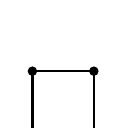
\begin{tikzpicture}[scale=0.78, line width=0.9pt, baseline=-0.5ex]
  \draw (0,0) -- (1,0) -- (1,1) -- (0,1) -- cycle;
  \foreach \p in {(0,0),(1,0),(1,1),(0,1)} \fill \p circle (2.2pt);
\end{tikzpicture}\\[3pt]
\textbf{2:}\;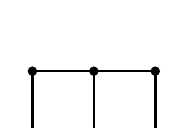
\begin{tikzpicture}[scale=0.78, line width=0.9pt, baseline=-0.5ex]
  \draw (0,0) -- (1,0) -- (1,1) -- (0,1) -- cycle;
  \draw (1,0) -- (2,0) -- (2,1) -- (1,1);
  \foreach \p in {(0,0),(1,0),(2,0),(0,1),(1,1),(2,1)} \fill \p circle (2.2pt);
\end{tikzpicture}\\[3pt]
\textbf{3:}\;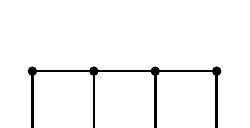
\begin{tikzpicture}[scale=0.78, line width=0.9pt, baseline=-0.5ex]
  \draw (0,0) -- (1,0) -- (1,1) -- (0,1) -- cycle;
  \draw (1,0) -- (2,0) -- (2,1) -- (1,1);
  \draw (2,0) -- (3,0) -- (3,1) -- (2,1);
  \foreach \p in {(0,0),(1,0),(2,0),(3,0),(0,1),(1,1),(2,1),(3,1)} \fill \p circle (2.2pt);
\end{tikzpicture}

\begin{enumerate}[label=(\alph*)]
  \item Draw the next pattern (4 squares in a row).
  \drawbox{2.8cm}
  \item Copy and complete the table.

  \patterntable{$S$}{$M$}{7}{{},1,2,3,4,5,12}

  \item Construct a formula for the number of matches ($M$) needed for any number of squares ($S$).
  \anshere
  \item If a row had 40 squares, how many matches would be needed?
  \anshere
  \item If a row had 75 squares, how many matches would be needed?
  \anshere
\end{enumerate}

\columnbreak

\section*{Question 2 -- Hexagonal Picnic Tables}

A campsite joins hexagonal picnic tables end to end in a row, as shown below (each dot is a
seat). When two tables are pushed together, the shared side can no longer seat anyone.

\noindent\textbf{1:}\;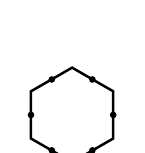
\begin{tikzpicture}[scale=0.60, line width=0.9pt, baseline=-0.5ex]
  \draw (0.87,0.5) -- (0,1) -- (-0.87,0.5) -- (-0.87,-0.5) -- (0,-1) -- (0.87,-0.5) -- cycle;
  \foreach \p in {(0.43,0.75),(-0.43,0.75),(-0.87,0),(-0.43,-0.75),(0.43,-0.75),(0.87,0)}
    \fill \p circle (2pt);
\end{tikzpicture}\\[3pt]
\textbf{2:}\;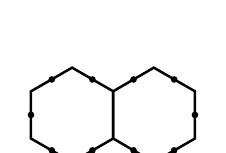
\begin{tikzpicture}[scale=0.60, line width=0.9pt, baseline=-0.5ex]
  \draw (0.87,0.5) -- (0,1) -- (-0.87,0.5) -- (-0.87,-0.5) -- (0,-1) -- (0.87,-0.5) -- cycle;
  \draw (2.6,0.5) -- (1.73,1) -- (0.87,0.5) -- (0.87,-0.5) -- (1.73,-1) -- (2.6,-0.5) -- cycle;
  \foreach \p in {(0.43,0.75),(-0.43,0.75),(-0.87,0),(-0.43,-0.75),(0.43,-0.75),
                  (2.16,0.75),(1.30,0.75),(1.30,-0.75),(2.16,-0.75),(2.6,0)}
    \fill \p circle (2pt);
\end{tikzpicture}\\[3pt]
\textbf{3:}\;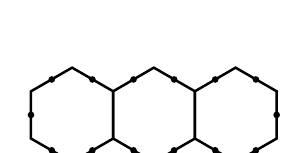
\begin{tikzpicture}[scale=0.60, line width=0.9pt, baseline=-0.5ex]
  \draw (0.87,0.5) -- (0,1) -- (-0.87,0.5) -- (-0.87,-0.5) -- (0,-1) -- (0.87,-0.5) -- cycle;
  \draw (2.6,0.5) -- (1.73,1) -- (0.87,0.5) -- (0.87,-0.5) -- (1.73,-1) -- (2.6,-0.5) -- cycle;
  \draw (4.33,0.5) -- (3.46,1) -- (2.6,0.5) -- (2.6,-0.5) -- (3.46,-1) -- (4.33,-0.5) -- cycle;
  \foreach \p in {(0.43,0.75),(-0.43,0.75),(-0.87,0),(-0.43,-0.75),(0.43,-0.75),
                  (2.16,0.75),(1.30,0.75),(1.30,-0.75),(2.16,-0.75),
                  (3.89,0.75),(3.03,0.75),(3.03,-0.75),(3.89,-0.75),(4.33,0)}
    \fill \p circle (2pt);
\end{tikzpicture}

\begin{enumerate}[label=(\alph*)]
  \item Draw the next pattern (4 hexagonal tables joined in a row).
  \drawbox{3.0cm}
  \item Copy and complete the table below.

  \patterntable{$T$}{$C$}{7}{{},1,2,3,4,5,25}

  \item Construct a formula for the number of seats ($C$) needed for any number of tables ($T$).
  \anshere
  \item If the campsite joined 40 tables in a row, how many seats would there be?
  \anshere
  \item If the campsite needed to seat 70 people in a single row of joined tables, how many
    tables would be needed?
  \anshere
\end{enumerate}

\end{multicols}

\newpage

\begin{multicols}{2}

\section*{Question 3 -- Matchstick Towers}

This pattern shows the number of matchsticks needed to make a row of joined towers (each
tower is 1 matchstick wide and 3 matchsticks tall). Neighbouring towers share a whole wall --
3 matchsticks' worth of overlap.

\noindent\textbf{1:}\;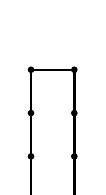
\begin{tikzpicture}[scale=0.55, line width=0.9pt, baseline=-0.5ex]
  \draw (0,0) -- (1,0); \draw (0,3) -- (1,3);
  \draw (0,0) -- (0,3); \draw (1,0) -- (1,3);
  \foreach \x in {0,1} \foreach \y in {0,1,2,3} \fill (\x,\y) circle (2.2pt);
\end{tikzpicture}\\[3pt]
\textbf{2:}\;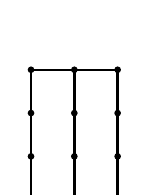
\begin{tikzpicture}[scale=0.55, line width=0.9pt, baseline=-0.5ex]
  \draw (0,0) -- (2,0); \draw (0,3) -- (2,3);
  \draw (0,0) -- (0,3); \draw (1,0) -- (1,3); \draw (2,0) -- (2,3);
  \foreach \x in {0,1,2} \foreach \y in {0,1,2,3} \fill (\x,\y) circle (2.2pt);
\end{tikzpicture}\\[3pt]
\textbf{3:}\;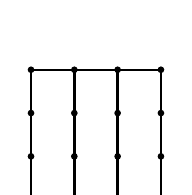
\begin{tikzpicture}[scale=0.55, line width=0.9pt, baseline=-0.5ex]
  \draw (0,0) -- (3,0); \draw (0,3) -- (3,3);
  \draw (0,0) -- (0,3); \draw (1,0) -- (1,3); \draw (2,0) -- (2,3); \draw (3,0) -- (3,3);
  \foreach \x in {0,1,2,3} \foreach \y in {0,1,2,3} \fill (\x,\y) circle (2.2pt);
\end{tikzpicture}

\begin{enumerate}[label=(\alph*)]
  \item Draw the next pattern (4 towers in a row).
  \drawbox{3.0cm}
  \item Copy and complete the table.

  \patterntable{$T$}{$M$}{7}{{},1,2,3,4,5,20}

  \item Construct a formula for the number of matches ($M$) needed for any number of towers ($T$).
  \anshere
  \item If a row had 30 towers, how many matches would be needed?
  \anshere
  \item If a row had 60 towers, how many matches would be needed?
  \anshere
\end{enumerate}

\columnbreak

\section*{Question 4 -- Paper Cutting (Geometric)}

A square sheet of paper is cut with straight vertical cuts, each one cutting every piece made
so far exactly in half. This pattern is \emph{geometric}, not linear: the number of pieces is
\emph{multiplied} by the same amount at each stage.

\noindent\textbf{1:}\;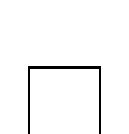
\begin{tikzpicture}[scale=0.9, line width=0.9pt, baseline=-0.5ex]
  \draw (0,0) rectangle (1,1);
\end{tikzpicture}\\[3pt]
\textbf{2:}\;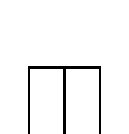
\begin{tikzpicture}[scale=0.9, line width=0.9pt, baseline=-0.5ex]
  \draw (0,0) rectangle (1,1);
  \draw (0.5,0) -- (0.5,1);
\end{tikzpicture}\\[3pt]
\textbf{3:}\;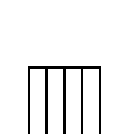
\begin{tikzpicture}[scale=0.9, line width=0.9pt, baseline=-0.5ex]
  \draw (0,0) rectangle (1,1);
  \draw (0.25,0) -- (0.25,1);
  \draw (0.5,0) -- (0.5,1);
  \draw (0.75,0) -- (0.75,1);
\end{tikzpicture}

\begin{enumerate}[label=(\alph*)]
  \item Draw the next pattern (stage 4).
  \drawbox{2.4cm}
  \item Copy and complete the table below.

  \patterntable{$n$}{$P$}{6}{1,2,3,4,5,7}

  \item Construct a formula for the number of pieces ($P$) at stage $n$. (Hint: write a few
    terms as powers of the ratio you found above.)
  \anshere
  \item How many pieces are there at stage 8?
  \anshere
  \item How many pieces are there at stage 10?
  \anshere
\end{enumerate}

\end{multicols}

\newpage

\begin{multicols}{2}

\section*{Section 5 -- Sequences in Words}

\subsection*{Word problem 1}

A candle is 24~cm tall when it is lit. Every hour it burns down, it loses 4~cm of height.

\begin{enumerate}[label=(\alph*)]
  \item Copy and complete the table below, using the words above.

  \patterntable{$h$}{$H$}{6}{{},1,2,3,4,5}

  \item Construct a formula for the height ($H$) after $h$ hours.
  \anshere
  \item After how many hours does the candle burn out completely (height $=0$)?
  \anshere
  \item Your formula gives a height for $h=8$. Work it out, then explain why this answer
    doesn't make sense for the real candle.
  \anshere
\end{enumerate}

\columnbreak

\subsection*{Word problem 2}

A chess club has 15 members at the start of the year. Every week, 4 new people join the club
(and nobody leaves).

\begin{enumerate}[label=(\alph*)]
  \item Copy and complete the table below, using the words above.

  \patterntable{$w$}{$M$}{7}{{},1,2,3,4,5,25}

  \item Construct a formula for the number of members ($M$) after $w$ weeks.
  \anshere
  \item How many members would there be after 10 weeks?
  \anshere
  \item After how many weeks would the club have 99 members?
  \anshere
\end{enumerate}

\end{multicols}

\newpage

\begin{multicols}{2}

\section*{Section 6 -- Just the Numbers}

\subsection*{Pattern A}

\begin{center}
\begin{tabular}{|c|c|c|c|c|c|}
  \hline
  $n$ & 1 & 2 & 3 & 4 & 5 \\
  \hline
  $y$ & 5 & 9 & 13 & 17 & 21 \\
  \hline
\end{tabular}
\end{center}

\begin{enumerate}[label=(\alph*)]
  \item Find a formula for $y$ in terms of $n$.
  \anshere
  \item Describe a real-life situation this sequence could represent.
  \ansprose
  \item Use your formula to find the 15th term.
  \anshere
\end{enumerate}

\subsection*{Pattern B}

\begin{center}
\begin{tabular}{|c|c|c|c|c|c|}
  \hline
  $n$ & 1 & 2 & 3 & 4 & 5 \\
  \hline
  $y$ & 50 & 45 & 40 & 35 & 30 \\
  \hline
\end{tabular}
\end{center}

\begin{enumerate}[label=(\alph*)]
  \item Find a formula for $y$ in terms of $n$.
  \anshere
  \item Describe a real-life situation this sequence could represent.
  \ansprose
  \item Use your formula to find the 10th term.
  \anshere
\end{enumerate}

\columnbreak

\subsection*{Pattern C}

\begin{center}
\begin{tabular}{|c|c|c|c|c|c|}
  \hline
  $n$ & 1 & 2 & 3 & 4 & 5 \\
  \hline
  $y$ & 3 & 6 & 12 & 24 & 48 \\
  \hline
\end{tabular}
\end{center}

\begin{enumerate}[label=(\alph*)]
  \item Find a formula for $y$ in terms of $n$.
  \anshere
  \item Describe a real-life situation this sequence could represent.
  \ansprose
  \item Use your formula to find the 8th term.
  \anshere
\end{enumerate}

\subsection*{Pattern D}

\begin{center}
\begin{tabular}{|c|c|c|c|c|c|}
  \hline
  $n$ & 1 & 2 & 3 & 4 & 5 \\
  \hline
  $y$ & 8 & 8 & 8 & 8 & 8 \\
  \hline
\end{tabular}
\end{center}

\begin{enumerate}[label=(\alph*)]
  \item Find a formula for $y$ in terms of $n$.
  \anshere
  \item Describe a real-life situation this sequence could represent.
  \ansprose
  \item Use your formula to find the 20th term.
  \anshere
\end{enumerate}

\end{multicols}

\end{document}
